\documentclass[11.5pt]{sig-alternate} % sets document style to sig-alternate
% packages
% typesetting
%\usepackage{dirtytalk} % typset quotations easier (\say{stuff})
\usepackage{hanging} % hanging paragraphs
\usepackage[defaultlines=3,all]{nowidow} % avoid widows
\usepackage[pdfpagelabels=false]{hyperref} % produce hypertext links, includes backref and nameref
\usepackage{xurl} % defines url linebreaks, loads url package
\usepackage{microtype}
%\usepackage[super]{nth} % easily create superscript ordinal numbers with \nth{x}\
\usepackage{enumitem}
% layout
\usepackage{enumitem} % control layout of itemize, enumerate, description
\usepackage{fancyhdr} % control page headers and footers
\usepackage{float} % improved interface for floating objects
%\usepackage{multicol} % intermix single and multiple column pages
% language
\usepackage[utf8]{inputenc} % accept different input encodings
\usepackage[english]{babel} % multilanguage support
% misc
\usepackage{graphicx} % builds upon graphics package, \includegraphics
%\usepackage{lastpage} % reference number of pages
%\usepackage{comment} % exclude portions of text (?)
\usepackage{xcolor} % color extensions
\usepackage[backend=biber, style=apa]{biblatex} % sophisticated bibliographies % necessary for HTML to display author info and date on abstract page
\usepackage{csquotes} % advanced quotations, makes biblatex happy
\usepackage{authblk} % support for footnote style author/affiliation
% tables and figures
\usepackage{tabularray}
%\usepackage{array} % extend array and tabular environments
\usepackage{caption} % customize captions in figures and tables (rotating captions, sideways captions, etc)
%\usepackage{cuted} % allow mixing of \onecolumn and \twocolumn on same page
\usepackage{multirow} % create tabular cells spanning multiple rows
%\usepackage{subfigure} % deprecated, support for manipulation of small figures
%\usepackage{tabularx} % extension of tabular with column designator "x", creates paragraph-like column whose width automatically expands
%\usepackage{wrapfig} % allows figures or tables to have text wrapped around them
%\usepackage{booktabs} % better rules
% dummy text
%\usepackage{blindtext} % blind text dummy text
%\usepackage{kantlipsum} % Kant style dummy text
\usepackage{lipsum} %lorem ipsum dummy text
% other helpful packages may be booktabs, longtable, longtabu, microtype

\pagestyle{fancy} % sets pagestyle to fancy for fancy headers and footers

% header and footer
% modern way to set header image
\renewcommand{\headrulewidth}{0pt} % defines thickness of line under header
\renewcommand{\footrulewidth}{0pt} % defines thickness of line above header
\setlength\headheight{80.0pt} % sets height between top margin and header image, effectively moves page contents down
\addtolength{\textheight}{-80.0pt} % seems to affect the lower height. maybe only works properly if footer numbers enabled?
\fancyhf{}
\fancyhead[CE, CO]{
\includegraphics[width=\textwidth]{headerImage.png}}
% footer
%\fancyfoot[LE,LO]{Article Title Here \\ DOI: }% left footer article title and doi
%\fancyfoot[CE,CO]{{}} % center footer empty
%\fancyfoot[RE,RO]{\thepage} % right footer page numbers
%\pagenumbering{arabic} % arabic (1, 2, 3) numbering in footer

\hypersetup{colorlinks=true,urlcolor=blue} % sets link color to blue
\urlstyle{same} % sets url typeface to same as rest of text

% set caption and figure to italics, label bold, left align captions, does not transfer to HTML
\DeclareCaptionFormat{custom}
{
    \textbf{\textit{\large #1#2}}\textit{\large #3} % #1 is the "Table 1" or "Figure 1" part, #2 is the separator (":"), #3 is the caption
}
\captionsetup{format=custom}
\captionsetup{justification = raggedright, singlelinecheck = false}

%this next bit is confusing, but essentially changes the width of the abstract. Seems to have been copied from this https://tex.stackexchange.com/questions/151583/how-to-adjust-the-width-of-abstract
\let\oldabstract\abstract
\let\oldendabstract\endabstract
\makeatletter %changes @ catcode to enable modification (in parsep)
\renewenvironment{abstract} %alters the abstract environment
{\renewenvironment{quotation}%
               {\list{}{\addtolength{\leftmargin}{1em} % change this value to add or remove length to the the default ?
                        \listparindent 1.5em%
                        \itemindent    \listparindent%
                        \rightmargin   \leftmargin%
                        \parsep        \z@ \@plus\p@}%
                \item\relax}%
               {\endlist}%
\oldabstract}
{\oldendabstract}
\makeatother %changes @ catcode to disable modification

\begin{document}

\title{Supplemental Online Learning Tools (SOLTs) to Support Deaf and Hard of Hearing Students in Introductory Statistics Courses}

\author[1]{\large \color{blue}Jacqueline McClive}
\author[1]{\large \color{blue}Carol E. Marchetti}
\author[1]{\large \color{blue}Gary Blatto-Vallee}
\author[1]{\large \color{blue}Sue Foster}
\author[1]{\large \color{blue}Keith Mousley}
\author[1]{\large \color{blue}David Simkins}
\author[1]{\large \color{blue}Jane Jackson}
\affil[1]{Rochester Institute of Technology}


\toappear{}
%% ABSTRACT
\maketitle
\begin{@twocolumnfalse} 
\begin{abstract}
\item 
\textit {Research in most Science, Technology, Engineering, and Mathematics (STEM) disciplines uses statistical methods. Thus as students develop into research scientists, introductory statistics serves as a gateway course. If students struggle to incorporate statistics into their knowledge base, they may be effectively kept from careers that rely on statistics. Students who are Deaf or Hard-of-Hearing (DHH) learn differently and thus may lag behind their hearing counterparts in mainstream classrooms. In part, a gap in language knowledge can impede the understanding of statistics topics. What is a variable? What does it mean to have a distribution? With sign language interpreters and other support services, many mainstream instructors believe that DHH students have equal access to learning in their classrooms. Yet variations of instructional skill, interpreter knowledge of the discipline, and the lack of alternative representations of content often result in access that falls short of "equal". This paper describes the work of a team of faculty and student researchers seeking best practices for creating supplemental online learning tools. Starting from a list of prioritized challenging topics in statistics, the team developed a number of strategies and produced a pilot set of instructional videos. Formative feedback led to revised videos, which provided a significant gain in knowledge for DHH students when shown in an experimental setting.}
\\ \\
Keywords: statistics, deaf, online, video
\end{abstract}
\end{@twocolumnfalse}

%% AUTHOR INFORMATION

\textbf{*Corresponding Author, Carol E. Marchetti}\\
\href{mailto: cemsma@rit.edu}{(cemsma@rit.edu)} \\
\textit{Submitted March 1, 2020 } \\
\textit{Accepted April 14, 2020} \\
\textit{Published online July 23, 2020} \\
\textit{DOI:10.14448/jsesd.12.0009} \\
\pagebreak
\clearpage

\begin{large}
\section*{INTRODUCTION}

As employers continue to increase their reliance on data, more universities and high schools (and even primary schools) have introduced statistics requirements. For example, the common core standard, adopted by forty-one U.S. states, includes “Develop understanding of statistical variability” as a Grade 6 requirement (National Governors Association Center for Best Practices, 2010). At the post-secondary level, 627,000 students took an introductory statistics course in 2015 (Blair, Kirmane, \& Maxwell, 2018). It is recognized that, with the rapid increase in available data, statistical education is more important than ever; statistical reasoning can help us can make informed decisions as we navigate our lives as citizens, employees, and family members (GAISE, 2016). If students struggle to incorporate statistics into their knowledge base, they may be effectively kept from careers that rely on statistics.

It’s estimated that 90\% of DHH children have hearing parents (Mitchell \& Karchmer, 2004). According to the National Association of the Deaf, some hearing parents of DHH children are told that signing is not needed or will interfere with learning speech (National Association of the Deaf, 2020), possible deterring some families from using ASL. As a visual language ASL has its own learning curve which, while hearing parents are mastering it, can pose challenges to providing linguistic-rich interaction and communication strategies that support language intake for their DHH children (Spencer \& Koester, 2016). Because of differing communication modes and a decreased ability to “overhear” conversations, children who are DHH often need to be directly taught skills that hearing children learn incidentally (Doyle \& Dye, 2002). As a result, the background knowledge that most hearing students bring into the classroom is unavailable to DHH students. If not addressed by classroom teachers, this becomes an obstacle to learning. 

Yosso (2005) makes that case that privileged groups create barriers for those without the same cultural capital, and that educational systems do not acknowledge or consider the cultural wealth of minority communities. Basic mathematics skills are an important factor in student success in introductory statistics (Johnson \& Kuennen, 2006), but DHH students learn mathematics differently and the instruction in mainstream classrooms may cause them to lag behind their hearing counterparts. At the pre-school level, Pagliaro \& Krizter (2013) found that DHH learners have more understanding of geometry and space, and less understanding of measurement and problem-solving, than hearing learners. In grades K-3, DHH students rely primarily on counting strategies to solve problems, while hearing students progress through a series of strategies (Pagliaro \& Ansell, 2012). Between classroom challenges and obstacles in testing, at age 18 students who are DHH have a median mathematics problem-solving score at the 5th level on the Stanford 10 Achievement Test (Qi \& Mitchell, 2011).

In the same vein, the educational system often yields DHH students with weaker English language skills than their hearing peers (Schley \& Albertini, 2005). Qi \& Mitchell (2011) found that 18-year-old DHH students had a median score at the 3rd grade level on the Stanford 10 Reading Comprehension and Reading Vocabulary Tests. This gap in language knowledge can also impede the understanding of statistics topics. What is a variable? What does it mean to have a distribution? What is the difference between a population mean and a sample mean? Students with lower level English skills may need more time and processing (Bay-Williams \& Herrera, 2007; Bose \& Choudhury, 2010). In a math or statistics class, any student that is struggling with the language in a given problem might miss mathematics learning due to the time spent focused on the English (Sharma, 2016). Kelly \& Mousley (2001) found that DHH college students experienced difficulty with mathematical problem-solving due to these same language issues. On top of this, technical language and mathematical vocabulary that are essential to succeed in future mathematics learning, as well as in future careers, are often a challenge to DHH students (Borgiolo, 2008; Hoffert, 2009; Morgan, Craig, Schuette, \& Wagner, 2014; Neville-Barton \& Barton, 2005; Xi \& Yeping, 2008). Many DHH students who are not native English speakers must seek out resources beyond the classroom, such as tutors, text materials, and instructor time (Marschark, Sapere, Convertino, \& Seewagen, 2005), to master technical terminology.

Project Thinking CAP: Communication, Access, \& Persistence Among Deaf and Hard of Hearing Students in Foundational Statistics Courses aimed to investigate the potential of Supplemental Online Learning Tools (SOLTs) to enhance the academic success of DHH students in foundational statistics courses. SOLTs integrate visual and textual representations of concepts with explanations in sign language, voice and captioning. Core objectives include 1) develop a pilot collection of SOLTs and 2) test the efficacy of these videos. The design of each SOLT incorporates a series of micro-videos that breaks a topic into parts, and explains the terms and concepts needed to understand the topic. These videos are distinct from other similar resources in that they are created for DHH students, not simply adapted from resources created for a hearing audience.

By law, educational institutions must provide reasonable and appropriate accommodations to ensure equal access to education for students with disabilities. It is a common misconception that adding captioning or interpreting to a video solves any problems of accessibility for DHH viewers. While such accommodations provide \textit{communication access}, they do not necessarily ensure access to information, which often includes multiple communication modes and/or multiple representations of concepts so that individuals understand the content of the message. DHH students report classroom communication in general as a challenge (Stinson, Liu, Saur, \& Long, 1996). A phenomenon known as visual crowding can cause students to feel overwhelmed and confused. In a standard "accessible" classroom, a DHH student may have to attend to an interpreter, a PowerPoint Presentation displayed by the instructor, writing on a board at the front of the classroom, captioning, and/or discussions held between other students in the class. 

The interpretation process is complex for interpreters of both spoken languages and signed languages. Even with a highly-skilled and experienced interpreter, mistakes can and will be made. Interpretation errors, known as miscues, can distort the message being delivered to the consumer in a number of ways. According to The Cokely Model (Cokely, 1992), miscues can be grouped into five categories: omissions, additions, substitutions, intrusions, and anomalies. Omissions occur when information is missing from the interpretation. Additions happen when the interpreter mistakenly includes their own input. If parts of the message are inaccurately changed, that is considered a substitution. If features of the source language appear in the target language message, an intrusion has occurred. Lastly, anomalies are characterized by a meaningless interpretation. 

It should also be noted that commonly there is delay in the flow of communication to DHH students who are relying on an interpreter. Interpreters make use of lag time, a delay in their interpretation for appropriate processing from one language to another. The processing and re-communication time involved in interpreting makes it challenging for DHH students to ask questions or interact in the classroom which may result in the student becoming passive (Saur, Layne, Hurley, \& Opton, 1986). However, by pausing for 10 seconds before calling on any student to answer a question, instructors can better accommodate students who rely on interpreting, as well as others who may benefit from additional time to process the question (Braun, et al., 2018). 

Finally, we must acknowledge that “interpreting cannot duplicate its source” (Marschark, et al., 2005, p. 76). The quality of classroom interpreting is affected by the interpreter’s qualification and comfort with the content (Braun, et al., 2018). If an interpreter lacks knowledge of discipline-specific language, this may cause issues with conveying the concept, especially when the term has a different common meaning. For example, in statistics the word “significant” can be confusing due to its multiple meanings (Rangecroft, 2002). Students may already be aware of the common meaning (important); fewer have seen its appearance in a mathematical or scientific context (significant figures), which still differs from its statistical meaning (data that are unlikely to occur by chance). Direct instruction in sign language could be a solution, but that is yet to be proven, and is not a feasible solution in many university contexts, where the number of DHH students is not sufficient to justify hiring instructors with both content mastery and ASL fluency.

\section*{METHODS}

\subsection*{Overview}

This study was conducted at Rochester Institute of Technology (RIT), a large private university comprised of nine colleges, one of which is the National Technical Institute for the Deaf (NTID). As such, RIT has approximately 1400 DHH students enrolled in classes each term, about 500 of whom are registered in mainstream courses within the other colleges of RIT; that is, courses that are not strictly for NTID students and where the instructors do not teach using American Sign Language (ASL). The introductory statistics course which provides the basis for this research is taught in RIT’s College of Science.

In seeking best practices for supplemental online learning tools, the research team first selected topics, developed pilot videos, and conducted focus groups, leading to the creation of a set of videos. An appropriate assessment tool was needed to determine effectiveness of the videos, thus one was developed with the goal of testing statistical knowledge rather than English reading skills. Once the assessment tool was ready, a one-group pre/posttest experiment was conducted.

\subsection*{Topic Selection \& Pilot Videos}

The research team first identified and prioritized topics for which SOLTs would be created by developing criteria and measures with which to evaluate the topics within the introductory statistics course. Statistical concepts were selected using multiple data sources and encompass concepts that are built upon throughout the introductory statistics course. The selection process incorporated the following:

\begin{itemize}
    \item Criteria: Topic selection for the first SOLT used two main criteria – scope of student impact and the degree to which the concept is foundational.
    \item Measures: We identified measureable quantities for each criterion.
    \item Data Sources: Sources of data were specified for each measureable quantity.
\end{itemize}

Once an initial topic was chosen, visuals, English words, and signs were thoughtfully selected to convey the concept to an audience of DHH college students. Two versions of the initial video were created – one with a mainstream model of hearing instructor and ASL interpreter, the other with direct instruction in ASL by a deaf instructor.

\subsection*{Focus Groups}

The two pilot videos were reviewed by two focus groups for accessibility. Focus group participants consisted of a total of nine DHH students with a variety of communication and learning preferences, all of whom had taken introductory statistics. The order in which the videos were shown differed for the two focus group sessions. Following each video, participants were asked to provide feedback via a written form followed by an open discussion. The form was not interpreted question by question into ASL, but participants could and did request clarification as they completed the form. The open discussion, led by a member of the research team, went through the same questions one-by-one asking about the pace, pictures, animations, captions, and color choices, as well as what participants liked or did not like about the video. Audio recording captured spoken comments as well as voice-interpreted signed comments. The audio recordings were transcribed and analyzed. Findings from the analysis were used in revision of the initial videos and creation of further videos. In all, a set of five SOLT videos were developed for foundational topics in introductory statistics. 

\subsection*{Assessment Tools}

An online tool was developed to assess statistics learning on the five topics included in the SOLTs. To get started, the team reviewed banks of test questions from six introductory statistics textbooks and test questions from several statistics instructors at our institution. We then developed questions with the goal of testing statistical knowledge rather than English reading skills. Thus we aimed for questions that would be equally difficult for Hearing and DHH students, at a reading level at or below 8th grade, and containing sentence structure that is easy for ASL users to follow. In all, 44 pilot questions in multiple-choice format were developed. We recruited 72 students (36 DHH, 36 hearing) to test the pilot questions by offering free pizza in exchange for taking the exam (see Figure 1 for demographics). About 72\% of the participants were male (similar to the percentage of male students at RIT), and about 78\% of participants reported English as their native (primary) language. Approximately 47\% reported having a prior or current course in statistics (including high school statistics such as Advanced Placement), with a higher percentage among the hearing participants (61\% as compared to 33\% of DHH participants).

\begin{figure}[h]
    \centering
    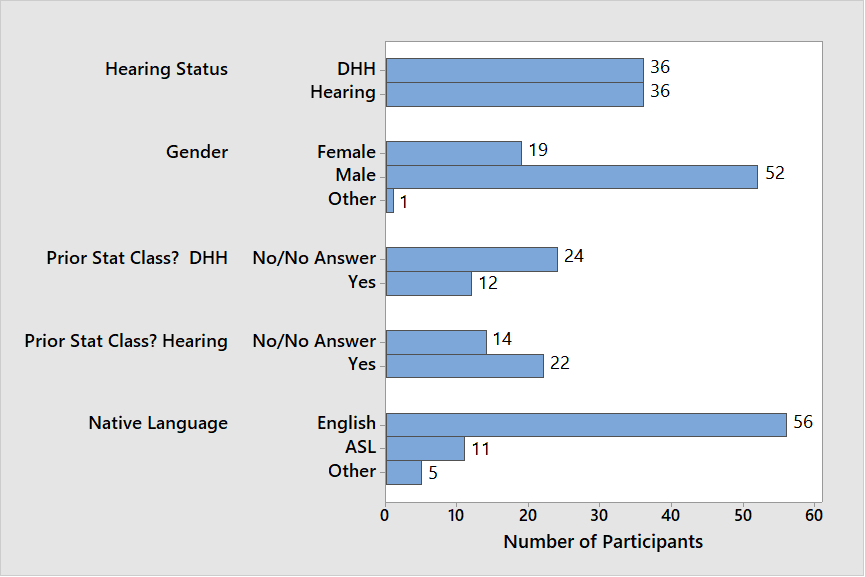
\includegraphics[width=1\linewidth]{Fig_1.png}
    \caption{Demographics of Pilot-Question Participants (n = 72)}
\end{figure}

\begin{itemize}
    \item From the test results, the team statistician (PhD and Professor of Statistics) suggested questions to eliminate on the basis of
    \item Statistical significance for the difference between \% correct for DHH vs Hearing,
    \item Difficulty level too low (over 60\% of DHH and 60\% of Hearing answered correctly), or
    \item Discrimination too low (low correlation between question correct answer and total score).
\end{itemize}

After review with the complete research team, a final set of twenty multiple-choice questions was established, with four questions on each of the five video topics. These questions served as both a pre- and post-test, administered on computer. The twenty questions were organized by topic, with topics presented in the same order each time, but within each topic the order of questions was randomized (assessment questions can be found in the appendix).

Additional assessments for math and reading skills were administered. The Wide Range Achievement Test-Fourth Edition (WRAT–4, Wilkinson \& Robertson, 2004) is a validated measure of reading, spelling, and basic math calculations. Only the Math Computation Subset was administered in this study, with math problems in addition, subtraction, multiplication, division, fractions, decimals, and algebra. The Test of Silent Contextual Reading Fluency–Second Edition (TOSCRF-2, Hammill, Wiederholt, \& Allen, 2014) measures reading comprehension and general reading ability. This test presents a student with a series of passages that increase in difficulty and asks them to determine individual words within those passages.

\subsection*{SOLT Assessment Procedure}

To assess learning as a result of watching the videos, DHH students familiar with ASL were recruited through flyers posted across campus. Nineteen DHH students were recruited and each student met with the lead researcher one-on-one. All instructions were provided in written form. The researcher provided any needed clarification about the instructions. Within an individual session lasting between 60 and 90 minutes, each student was asked to: 1) complete the pre-test, 2) view the set of five videos in a standard order, 3) complete the post-test and answer demographic questions, and 4) take the WRAT-4 and TOSCRF-2 assessments. Steps 1 – 3 were completed within an online system. Step 4 was completed with pen and paper.

Demographics and summaries of the reading and math assessments are presented in Figure 2. We asked if students were familiar with ASL, but we did not assess fluency nor did we ask students to assess themselves. Most of the participants (15/19) identified as Deaf; slightly more than half (11/19) identified as male; more than half (12/19) had previously taken a statistics course; and slightly less than half identified English as their native language. Age ranged from 19 – 50 years, with a mean of 24.5 years. Reading grade level, as measured with the TOSCRF-2, ranged from 3.0 to 13.0, with a mean of 7.5; math standard scores of the participants, as measured with the WRAT-4, had a range of 59-129 with a mean of 95.5. The correlation between reading grade level and math standard score was positive and moderately strong (r = 0.503). Average reading grade levels and math standard scores were not significantly different for those who identified English as their first language and those who identified ASL as their first language.

\begin{figure}[h]
    \centering
    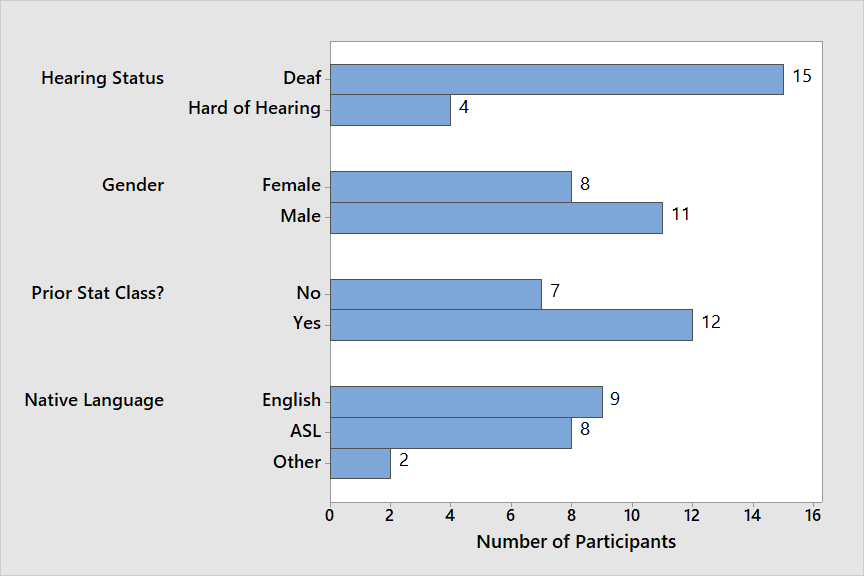
\includegraphics[width=1\linewidth]{Fig_2a.png}
\end{figure}

\begin{figure}[h]
    \centering
    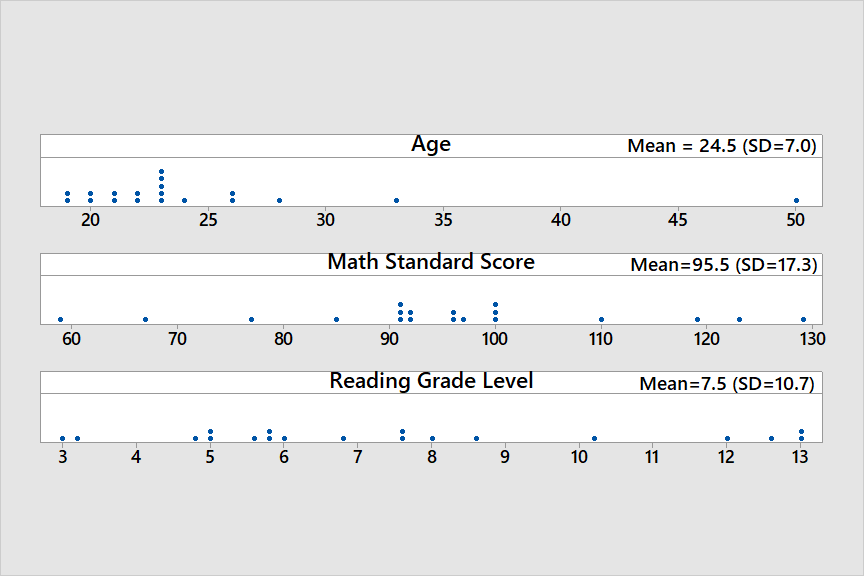
\includegraphics[width=1\linewidth]{Fig_2b.png}
    \caption{Demographics, Reading Grade Level, and Math Standard Scores of SOLT-Assessment Participants (n = 19)}
\end{figure}

\section*{RESULTS}

\subsection*{Creation of the Supplemental Online Learning Tools (SOLTs)}

What topics need SOLTs? A review of unit tests and final exams from past years yielded a list of topics where students struggled. At the same time, student-researchers on the team (DHH students who had completed the introductory statistics course) reviewed the course topic-by-topic, resulting in a list of “Top 5” difficult concepts. The most difficult topic appeared within hypothesis testing, that is identifying and describing Type I and Type II Errors. The combined complexity of English and statistics often left the students drowning in phrases such as, “The null hypothesis about the population is true, but there is sufficient sample evidence to reject it and conclude that the alternative hypothesis is true. Therefore a Type I Error was made.” Even for native English speakers, this is a dense and intricate thought process. As the project team broke this complex concept into several smaller topics (establishing hypotheses, interpreting the p-value, etc.), it seemed that many of the difficulties stemmed from identifying the data type. Hence, “Identifying Data Type” was selected as the first SOLT topic. This includes determination of population versus sample as well as categorical versus numerical. Identifying data type is critical in the selection of appropriate statistical techniques for a data set.

The design of each SOLT incorporates a series of micro-videos that breaks a topic into parts, and explains the terms and concepts needed to understand the topic. The first micro-video topic was “Population and Sample” for which two pilot versions were created. One video used slides with text and graphics, voice of the instructor and video of ASL interpretation (both provided by project team members with experience as statistics instructor and interpreter), similar to the way in which DHH students in mainstream classes receive instruction. The other video used the same slides but incorporated video of a deaf team member (with experience teaching mathematics and tutoring statistics) providing “direct instruction” in ASL. Although the two formats may appear to be identical to an outside observer, they serve two different subsets of the DHH population, based upon communication preferences. 

\begin{figure}[h]
    \centering
    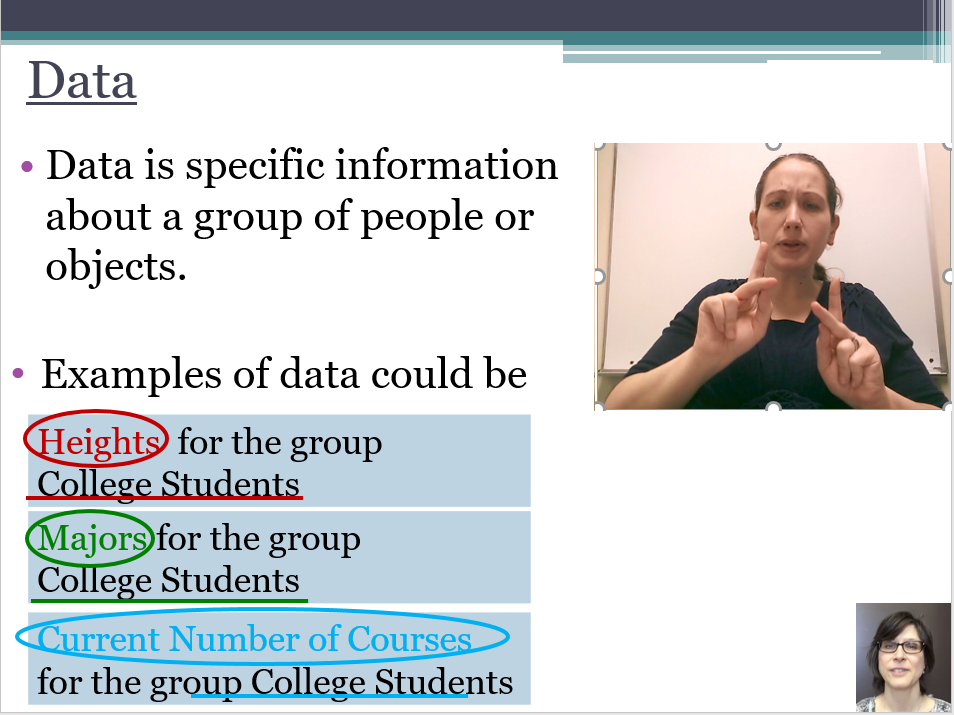
\includegraphics[width=1\linewidth]{Fig_3a.png}
\end{figure}

\begin{figure}[h]
    \centering
    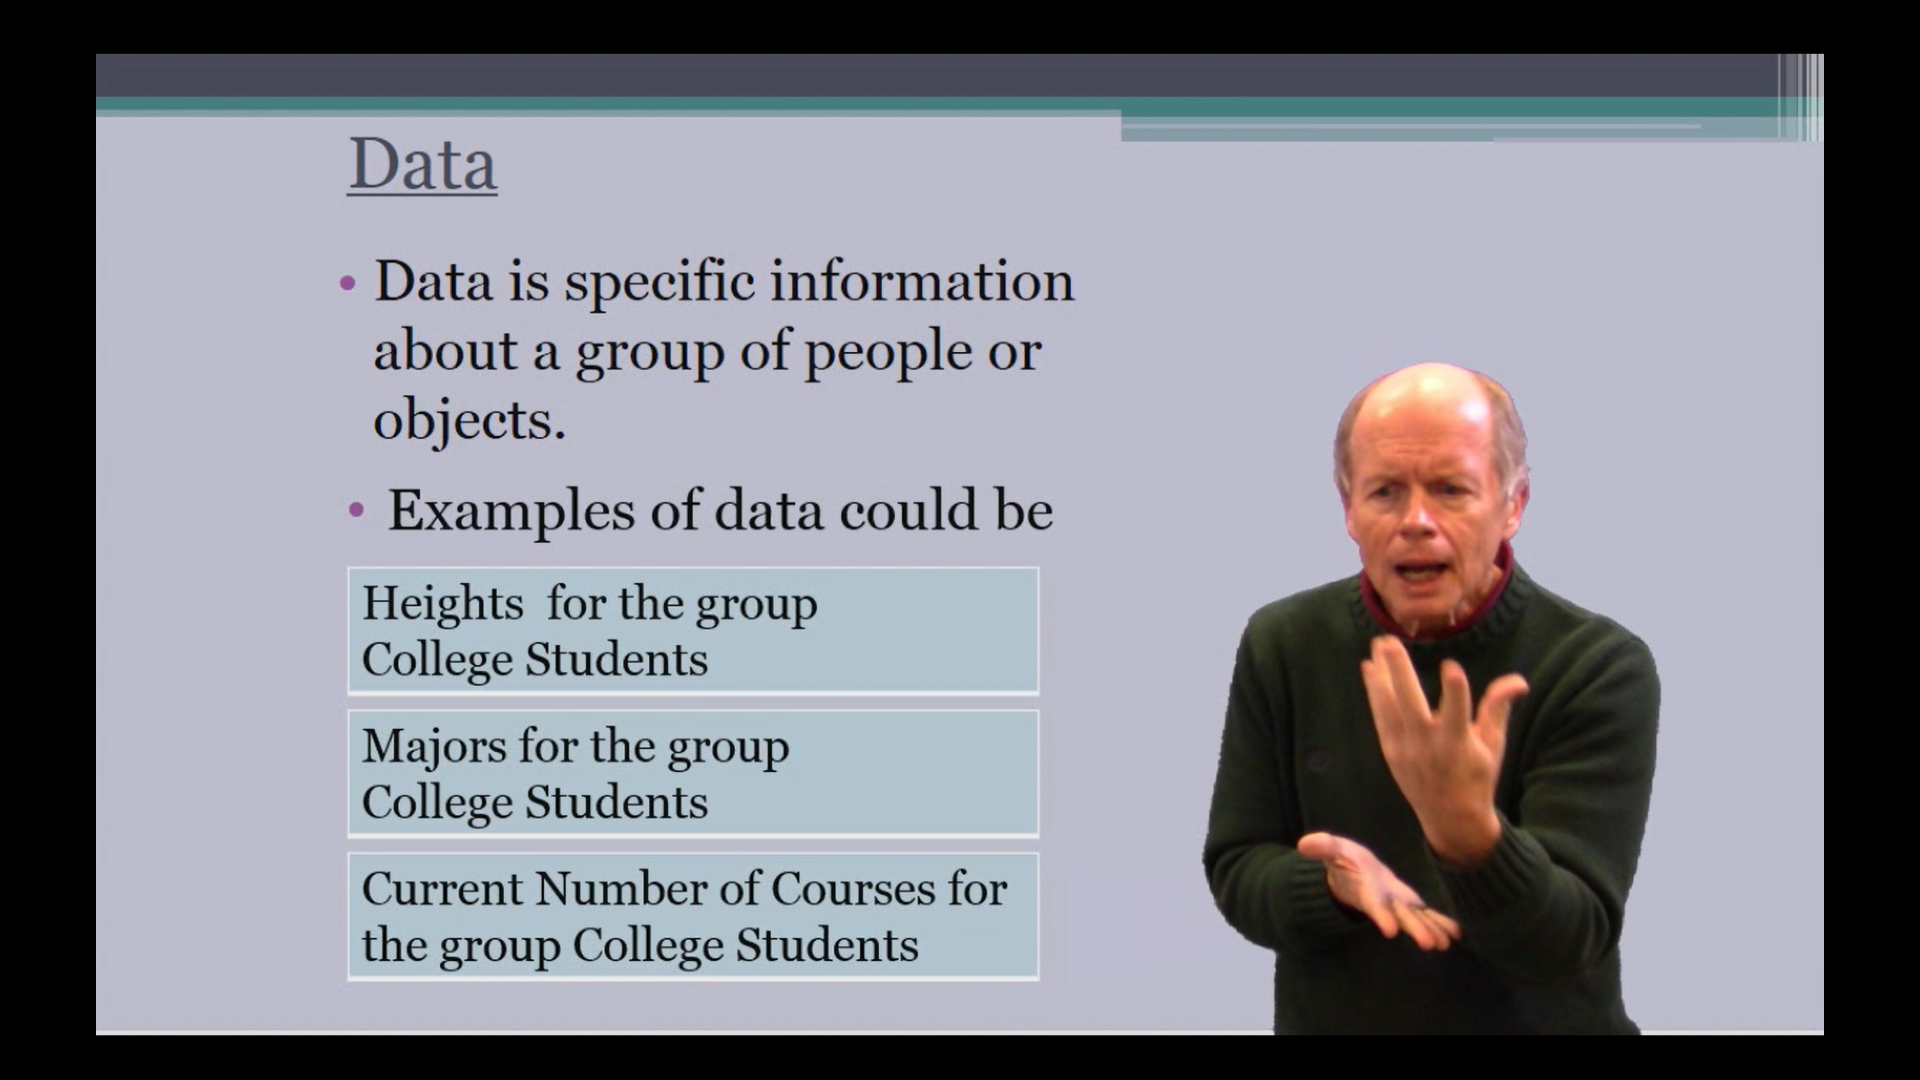
\includegraphics[width=1\linewidth]{Fig_3b.png}
    \caption{Screenshots from Instructor/Interpreter and Direct Instruction Pilot Videos}
\end{figure}

\subsection*{Student Feedback}

Analysis of the transcripts from the focus group sessions revealed the five themes described below.
Technical and design issues focused on pace, captioning, and interpreting. Focus group participants were very honest in providing feedback; one of them noted as we began to discuss what we defined as technological issues, "You know it’s really more than a technical problem." Participants shared both positive and negative feedback with equal enthusiasm. They identified technical and design issues that made it difficult for them to follow the first video, including issues of pace, captions, and interpreting. They weighed the balance between direct instruction and instruction mediated via interpreters, described the challenges in following both captions/interpreting and the visuals at the same time, and suggested fixes such as allowing more time for students to study an image before offering an explanation.

Difficulty in attending to multiple visual information sources simultaneously. The most critical challenge identified by students is one that has existed since instructors began to use multiple inputs when teaching - the virtually impossible task of attending to multiple visual information sources simultaneously. They felt overwhelmed with the pace and amount of material, especially in the instructor-interpreter video. The team designed this video to give students options for accessing the instructor's comments - interpreter, caption, direct/indirect instruction, etc. However, the use of multiple information channels, while offering choices to students, also made the learning task more difficult for some. Students had to choose which source to use, and were not always sure which to pick; "I wasn’t sure where to go first, should I watch the interpreter first or watch the caption first or maybe if I watch the interpreter first than watch the caption screen." With overlapping information venues many students attempted to take in multiple sources of input at the same time, making comprehension of the concept difficult.

Personal preferences for formatting. Students preferred different kinds of presentation, pace, highlighting, color themes, instruction, etc. For example, they expressed a variety of preferences regarding where captions would appear, at what rate, and how long they should remain on the screen. Some preferred direct instruction, some interpreted instruction, and others did not care which approach was used. This suggests that modifications to the tool that provide users with options to customize their interaction with the video tool would be considered an enhancement.

General preference for direct instruction. Overall students preferred the direct instruction video over the interpreted instruction video. They found it generally easier to use and more visually friendly. They offered suggestions regarding how to improve the videos and proposed that the team go through their points one by one and prioritize them. One student commented, “I really like having the direct communication with the instructor and seeing how he actually interacted with the PowerPoint slide itself. That was great to see how — what he was talking about showed up on the screen.”

Positive feelings about being asked to provide feedback. Students were very pleased that they were invited to participate in evaluating the videos. They felt their input was important and wished that this format was used more often by faculty in development of learning tools. In the words of one student, “I'm really happy that you’re getting student feedback... that you're not just going ahead with just faculty and that you're taking the time to see what students actually want and what they would think about it. I like that a lot. So thank you.”

During the discussion, students also offered their thoughts about engagement. They would like an experience that is more interaction and less passive. They also described the need for feedback on their understanding. This quote from one student aptly describes the consensus, “[This] could be more interesting and more fun and engaging… You could do different game [with] questions [and get] more creative.” 

\subsection*{Creating a Set of Videos}

Based on the focus group feedback, the original pilot videos were revised and additional videos were created. The direct-instruction ASL videos were filmed with a “green screen” making visuals larger and easier for the deaf instructor to reference. The instructor-interpreter/slide videos were adapted to allow students to control the pace by clicking when they are ready to move on, even clicking through the interpreter if not wanted. Eventually, it was decided to create only direct instruction videos. Of course, a benefit of this decision is that it reduced the scale of work that had doubled with making two versions of the video for each concept. More importantly, however, this is a significant symbolic gesture for DHH students. Most of the time DHH students use tools created for hearing students, accessible to them through accommodations. The videos we are creating are specifically for ASL users, accessible to hearing students through the addition of accommodations. In total, five videos were created using the same instructor – see Table 1 for the topic and length of each video. The videos are publicly available on the project’s YouTube channel, “Supplemental Online Learning Tools for Intro Stats”.

\begin{table}[ht]
\caption{Topics of SOLT videos}
\begin{tabular}{|l|c|}
\hline
\textbf{Topics} & \textbf{Length {min:sec}} \\ \hline
Population \& Sample & 3:33 \\ \hline
Categorical \& Numerical & 3:15 \\ \hline
Bias and Sampling & 4:37 \\ \hline
Mean and Standard Deviation & 5:48 \\ \hline
Proportion and Percentage & 9:24 \\ \hline
\end{tabular}
\end{table}

\subsection*{SOLT Assessment}

Do the SOLT videos improve learning for DHH students? Figure 4 displays the pre-test, post-test, and gain scores. Pre-test scores ranged from 10\% to 70\%, with a mean of 40.5\% (SD = 20.1\%), while post-test scores ranged from 20\% to 80\%, with a mean of 53.4\% (SD = 19.0\%). Pre-test and post-test scores each had a moderate correlation with the math standard score (r = 0.577, p < 0.05 and r = 0.552, p < 0.05 respectively), but were not significantly correlated with reading grade level. As expected, post-test had a strong, positive, linear relationship with pre-test score (r = 0.852, p < 0.001). Pre-test and post-test had no significant differences, on average, between those who identified English as their native language and those who identified ASL as their native language. Similarly, there were also no significant differences, on average, between those who previously took a statistics course and those who did not.

The increase from pre-test to post-test (or gain) varied from a low of 0\% to a maximum of 40\%. Average gain was 12.9\% (SD = 10.7\%), significantly different from zero (p < 0.0001), with a large effect size (Cohen's d = 1.20). Gain was not significantly correlated with either reading grade level or math standard score. There was also no significant difference, on average, between those who identified English as their first language and those who identified ASL as their first language, or between those who previously took a statistics course and those who did not.

\begin{figure}[h]
    \centering
    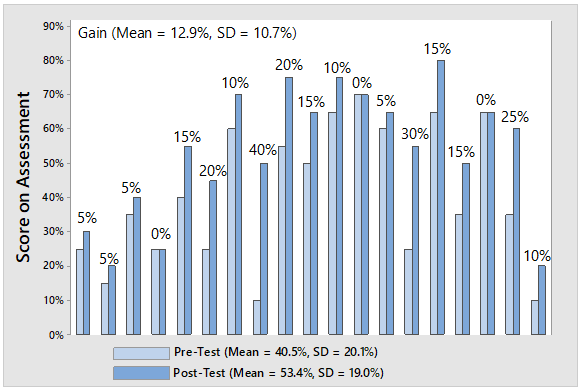
\includegraphics[width=1\linewidth]{Fig_4.png}
    \caption{Test Scores of SOLT Assessment Participants (n = 19)}
\end{figure}

The Proportion/Percentage topic had the highest pre-test score (57.9\%), while Population/Sam\-ple had the lowest pre-test score (22.4\%). The largest gains occurred for the Population/Sample topic (+21.1\%), followed by the Proportion/Per\-centage and Categorical/Numerical topics (+14-.5\% and +13.2\%, respectively). Figure 5 displays results for each of the five topics.

\begin{figure}[h]
    \centering
    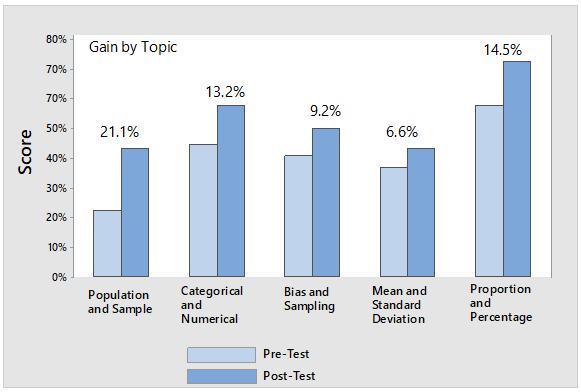
\includegraphics[width=1\linewidth]{Fig_5.png}
    \caption{Test Scores of DHH Video Assessment Participants by Topic (n = 19)}
\end{figure}

A limitation of this study is that no control group was included.  Thus, one cannot rule out that the act of taking the pre-test could have had an effect on post-test results. Since participants had recently read the same questions, familiarity with the vocabulary and situations presented may have influenced results.

\section*{DISCUSSION}

Ideally, DHH students would have the opportunity to learn statistics from a qualified instructor who is fluent in ASL. However, this type of professional is not readily available at most institutions of higher learning. The SOLTs were created bridge the gap for DHH students learning foundational statistics concepts in a mainstream environment. In our experimental setting, the students who participated in assessing the SOLTs showed an increase in statistics knowledge after viewing the videos. There are many video resources available online. Not all of them are accessible for students who are deaf or hard of hearing. This set of videos is unique in that they were created primarily for a DHH audience. And they have the potential for a larger improvement in learning than seen in the experiment when they are used to supplement a classroom experience. The positive results we observed indicate that more such resources are needed. Videos that provide direct instruction in ASL with voice interpretation could meet the needs of both DHH and hearing students. In addition, we wonder whether an experience that provides more engagement could be even more impactful.

According to Shapley (2000), students need to become self-directed and apply themselves using different strategies in order to succeed. Supplemental video resources can provide one strategy. Ideally, such learning tools would allow students to have choices and make mistakes while they learn independently. Active learning techniques, which include cooperative/collaborative learning, problem-based learning, peer instruction, inquiry-based learning, discovery learning, and technology-enhanced learning (Michael, 2006) have been shown to improve student outcomes (Freeman et al., 2014). Our focus group students indicated the desire for a more interactive learning experience. Thus, a new project objective emerged: Embed the SOLTs into an interactive web-based experience in which students can obtain, describe, and make inferences from samples within a relevant and appropriate context.

Our target population of DHH students are an ideal audience for an interactive educational experience because they tend to lag behind in English and math and often require visual presentation of concepts. By their nature, video games are very visual and can increase learning. According to De Freitas (2018), the research is “overwhelmingly positive” (p. 80) regarding the effectiveness of games as learning tools. Among adults in a medical setting, Ancker, Weber, \& Kukafka (2011) found that using a computer game-like graphic reduced differences in risk perception between low-numeracy and high-numeracy participants. In a postsecondary setting, Chow, Woodford, \& Maes (2011) investigated the use of an online version of the television game show “Deal or No Deal” to enhance student understanding of expected value in an introductory statistics course. One week after a lecture on expected value, students who played the game had a retention rate of 95\%, compared to 59\% for those who solved a problem on paper instead of playing the game.

\section*{FUTURE RESEARCH}

It is clear that investigation into some sort of learning game is warranted. Towards this end, the research team expanded to include specialists in game-based learning and development. Soon after, the project started planning a prototype for an interactive experience in the form of a digital-based learning game in which SOLTs could serve as stand-alone tools and tutorials within the interactive experience. This web-based tool would be mobile compatible and incorporate visuals that align with those in the SOLTs. Students may start by watching SOLTs or jump into the interactive experience and use the SOLTs as supports when needed. The framework for the interactive experience could eventually encompass multiple scenarios in which to play. The initial scenario is a student government election at the fictional Mars University. Within this environment, students select a candidate for whom they will campaign, take polls to gauge the student body’s preferences, and perform activities that attempt to sway opinions. 

\begin{figure}[h]
    \centering
    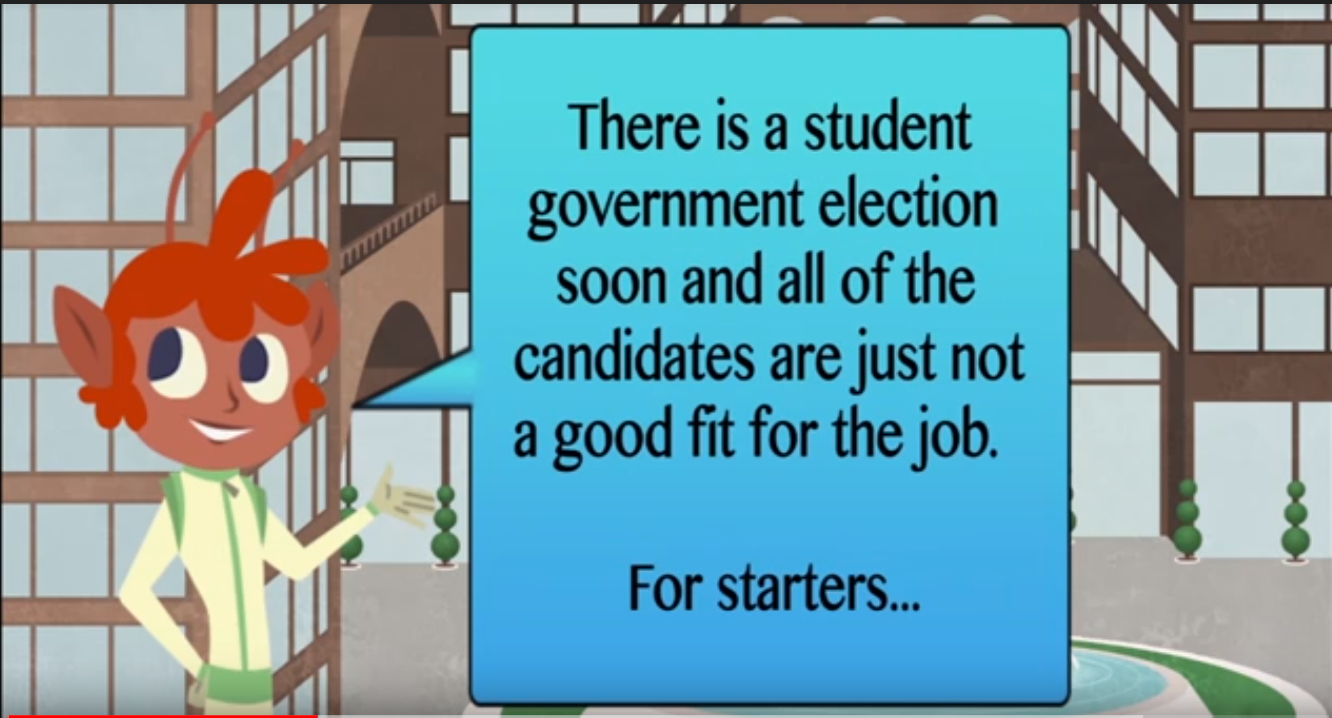
\includegraphics[width=1\linewidth]{Fig_6a.png}
\end{figure}

\begin{figure}[h]
    \centering
    
\includegraphics[width=1\linewidth]{Fig_6b.png}
    \caption{Screenshots from the MarsU game prototype}
\end{figure}

In what kind of framework might future statistical education games be based? An exploratory study by Dele-Ajayi, Strachan, \& Pickard (2016) used grounded theory to develop a framework of factors that support engagement with digital games. They identify clarity of goal and thematic/visual appeal as factors that trigger engagement, and rewards/feedback, social interaction, creativity, and challenge as factors that sustain engagement. Activity theory is another approach to designing educational games that also puts emphasis on the goal of the game. Activity is a purposeful interaction between subject and object, directed at a motive, and accomplished by a sequence of acts directed at a goal (Kaptelinin \& Nardi, 2006). An Activity-Theory-based Model of Serious Games (ATMSG) has been suggested by Carvalho, et al. (2015) to help designers connect game elements to each other and to the learning goals. More recently, Hanes and Stone (2018) have proposed using activity theory to design serious games for history education. 

A digital-based learning game in statistics could serve as a tool for students to interact with samples, creating a bridge between data concepts in an introductory statistics course and sampling activities within the game. With an activity theory approach, all components of the game would be connected to each other and to the learning goals around samples. Because the challenge of the learning games affects learning directly and also by increasing engagement, a learning game needs to maintain a challenge for the players as they develop abilities and knowledge while playing (Hamari et al., 2016).

We are still in the early stages of development and have much to learn about building digital-based learning games to serve the DHH population, from how to best explain the goal of the game without relying primarily on written English, to the types of icons that are culturally appropriate for this group. These types of tools have the potential to increase learning for DHH students in statistics, increase the number of DHH students who continue to pursue statistics or other STEM disciplines, and contribute to diversity within STEM workforce careers. With evidence to suggest that people learn more deeply with a combination of words and pictures than from words alone (Mayer, 2014), other learners may also benefit from the visual representation of complex concepts. The potential for the broader application of SOLTs and interactive experiences in other STEM subjects for DHH or other students may increase knowledge of how diverse groups of visual learners access complex concepts.

\section*{ACKNOWLEDGEMENTS}

Support for this research was provided by the National Science Foundation Improving Undergraduate STEM Education program under Award No. 1432566. Any opinions, findings, and conclusions or recommendations expressed in this material are those of the author(s) and do not necessarily reflect the views of the National Science Foundation.

\end{large}
\clearpage
\section*{REFRENCES}\par 
\leftskip 0.25in
\parindent -0.25in 
Ancker, J. S., Weber, E. U., \& Kukafka, R. (2011). Effects of game-like interactive graphics on risk perceptions and decisions. \textit{Medical Decision Making, 31}(1), 130-142. \url{https://doi.org/10.1177/0272989X10364847} 

Bay-Williams, J., \& Herrera, S. (2007). Is “just good teaching” enough to support the learning of English language learners? Insights from sociocultural learning theory. In W.G. Martin, M.E. Strutchens, \& P.C. Elliot (Eds.), \textit{The learning of mathematics: 69th NCTM yearbook} (pp. 43-63). Reston, VA: National Council of Teachers of Mathematics.

Blair, R., Kirmane, E. E., \& Maxwell, J. (2018). \textit{Statistical Abstract of Undergraduate Programs in the Mathematical Sciences in the United States: Fall CBMS 2015 Survey}. Providence, RI: American Mathematical Society. \url{https://www.ams.org/profession/data/cbms-survey/cbms2015-Report.pdf}

Borgioli, G. (2008). Equity for English language learners in mathematics classrooms. \textit{Teaching Children Mathematics, 15}(3), 185–191.

Bose, A., \& Choudhury, M. (2010). Language negotiation in a multilingual mathematics classroom: An analysis. In L. Sparrow, B. Kissane, \& C. Hurst (Eds.), \textit{Shaping the future of mathematics education} (pp. 93-100). Perth, WA, Australia: Mathematics Education Research Group of Australasia.

Braun, D. C., Clark, M. D., Marchut, A. E., Solomon, C. M., Majocha, M., Davenport, Z., Kushalnagar, R.S., Listman, J., Hauser, P.C., \& Gormally, C. (2018). Welcoming deaf students into STEM: Recommendations for university science education. \textit{CBE—Life Sciences Education, 17}(3), es10. \url{https://doi.org/10.1187/cbe.17-05-0081}

Carvalho, M. B., Bellotti, F., Berta, R., Gloria, A. D., Sedano, C. I., Hauge, J. B., Hu, J., \& Rauterberg, M. (2015). An activity theory-based model for serious games analysis and conceptual design. \textit{Computers \& Education, 87}, 166-181. \url{https://doi.org/10.1016/j.compedu.2015.03.023} 

Chow, A. F., Woodford, K. C., \& Maes, J. (2011). Deal or No Deal: using games to improve student learning, retention and decision-making. \textit{International Journal of Mathematical Education in Science and Technology, 42}(2), 259-264. \url{https://doi.org/10.1080/0020739X.2010.519796}

Cokely, D. (1992). \textit{Interpretation: A sociolinguistic model}. Burtonsville, MD: Linstok Press.

De Freitas, S. (2018). Are games effective learning tools? A review of educational games. \textit{Journal of Educational Technology \& Society, 21}(2), 74-84. \url{https://www.jstor.org/stable/26388380} 

Dele-Ajayi, O., Sanderson, J., Strachan, R., \& Pickard, A. (2016, October). Learning mathematics through serious games: an engagement framework. In \textit{2016 IEEE Frontiers in Education Conference Proceedings} (pp. 1-5). Piscataway, NJ: IEEE. \url{https://doi.org/10.1109/FIE.2016.7757401} 

Doyle, M., \& Dye, L. (2002). \textit{Mainstreaming the student who is deaf or hard of hearing. A guide for professionals, teachers and parents}. San Diego, USA: CCHAT Center. \url{https://www.handsandvoices.org/pdf/mainst\_cal.pdf}

Freeman, S., Eddy, S. L., McDonough, M., Smith, M. K., Okoroafor, N., Jordt, H., \& Wenderoth, M. P. (2014). Active learning increases student performance in science, engineering, and mathematics. \textit{Proceedings of the National Academy of Sciences, 111}(23), 8410-8415. \url{https://doi.org/10.1073/pnas.1319030111} 

GAISE College Report ASA Revision Committee (2016). \textit{Guidelines for assessment and instruction in statistics education college report 2016}. Alexandria, VA: American Statistical Association. \url{http://www.amstat.org/education/gaise}

Hamari, J., Shernoff, D. J., Rowe, E., Coller, B., Asbell-Clarke, J., \& Edwards, T. (2016). Challenging games help students learn: An empirical study on engagement, flow and immersion in game-based learning. \textit{Computers in Human Behavior, 54}, 170-179. \url{https://doi.org/10.1016/j.chb.2015.07.045} 

Hammill, D. D., Wiederholt, J. L., \& Allen, E. A. (2014). \textit{Test of silent contextual reading fluency}, second edition. Austin, TX: PRO-ED.

Hanes, L., \& Stone, R. (2018). A model of heritage content to support the design and analysis of video games for history education. \textit{Journal of Computers in Education}. \url{https://doi.org/10.1007/s40692-018-0120-2} 

Hoffert, S. B. (2009). Mathematics: The universal language? A teacher enumerates the challenges, strategies, and rewards of teaching mathematics to English language learners. \textit{Mathematics Teacher, 4}(2), 130-139.

Johnson, M., \& Kuennen, E. (2006). Basic math skills and performance in an introductory statistics course. \textit{Journal of Statistics Education, 14}(2). \url{https://doi.org/10.1080/10691898.2006.11910581}

Kaptelinin, V., \& Nardi, B. A. (2006). \textit{Acting with technology: Activity theory and interaction design}. Cambridge, MA: MIT Press.

Kelly, R., \& Mousley, K., (2001). Solving word problems: More than reading issues for deaf students. \textit{American Annals of the Deaf, 146}(3), 251-62. \url{https://www.jstor.org/stable/44393481} 

Marschark, M., Peterson, R., Winston, E. A., Sapere, P., Convertino, C. M., \& Monikowski, C. (Eds.) (2005). \textit{Sign language interpreting and interpreter education: Directions for research and practice}. Oxford (UK): Oxford University Press. 

Marschark, M., Sapere, P., Convertino, C., \& Seewagen, R. (2005). Access to postsecondary education through sign language interpreting. \textit{Journal of Deaf Studies and Deaf Education, 10}(1), 38-50. \url{https://doi.org/10.1093/deafed/eni002} 

Mayer, R. E. (2014). Incorporating motivation into multimedia learning. \textit{Learning and Instruction, 29}, 171–173. \url{http://doi.org/10.1016/j.learninstruc.2013.04.003}

Michael, J. (2006). Where's the evidence that active learning works? \textit{Advances in Physiology Education, 30}, 159-167. \url{https://doi.org/10.1152/advan.00053.2006} 

Mitchell, R., \& Karchmer, M. (2004). Chasing the mythical ten percent: Parental hearing status of deaf and hard of hearing students in the United States. \textit{Sign Language Studies, 4}(2), 138-163. \url{https://www.jstor.org/stable/26190985}

Morgan, C., Craig, T., Schuette, M., \& Wagner, D. (2014). Language and communication in mathematics education: An overview of research in the field. \textit{ZDM Mathematics Education, 46}(6), 843-853. \url{https://doi.org/10.1007/s11858-014-0624-9}

National Association of the Deaf (2020). \textit{Sign Language for Parents}. \url{https://www.nad.org/resources/early-intervention-for-infants-and-toddlers/information-for-parents/sign-language-for-parents/}

National Governors Association Center for Best Practices, (2010). \textit{Common Core State Standards for Mathematics}. Washington D.C.: Council of Chief State School Officers \url{www.corestandards.org/Math/Content/6/SP/}	

Neville-Barton, P., \& Barton, B. (2005). \textit{The relationship between English language and mathematics learning for non-native speakers}. Wellington, New Zealand: Teaching \& Learning Research Initiatives. \url{http://www.tlri.org.nz/sites/default/files/projects/9211\_summaryreport.pdf}

Pagliaro, C. M., \& Ansell, E. (2012). Deaf and hard of hearing students’ problem-solving strategies with signed arithmetic story problems. \textit{American Annals of the Deaf, 156}(5), 438-458. \url{https://www.jstor.org/stable/26235174}

Pagliaro, C. M., \& Kritzer, K. L. (2013). The math gap: A description of the mathematics performance of preschool-aged deaf/hard-of-hearing children. \textit{Journal of Deaf Studies and Deaf Education, 18}(2), 139-160. \url{https://doi.org/10.1093/deafed/ens070} 

Rangecroft, M. (2002). The language of statistics. \textit{Teaching Statistics, 24}(2), 34-37. \url{https://doi.org/10.1111/1467-9639.00080} 

Saur, R., Layne, C., Hurley, E., Opton, K. (1986). Dimensions of mainstreaming. \textit{American Annals of the Deaf, 131}(5), 325-330. \url{https://www.jstor.org/stable/44389851}

Schley, S., \& Albertini, J. (2005). Assessing the writing of deaf college students: Reevaluating a direct assessment of writing. \textit{Journal of Deaf Studies and Deaf Education, 10}(1), 96-105. \url{https://doi.org/10.1093/deafed/eni006} 

Shapley, P. (2000). On-line education to develop complex reasoning skills in organic chemistry. \textit{Journal of Asynchronous Learning Networks, 4}(2), 55-65.

Sharma, S. (2016). Language barriers in statistics education: Some findings from Fiji. \textit{International Journal of Learning, Teaching, and Educational Research, 15}(8), 23- 34. \url{http://ijlter.org/index.php/ijlter/article/view/682}

Spencer, P.E. and Koester L.S. (2016). \textit{Nurturing Language and Learning: Development of Deaf and Hard-of-Hearing Infants and Toddlers}. New York: Oxford University Press.

Stinson, M., Lui, Y., Saur, R., \& Long, G. (1996). Deaf college students’ perceptions of communication in mainstream classes. \textit{Journal of Deaf Studies and Deaf Education, 1}(1), 40-51. \url{https://doi.org/10.1093/oxfordjournals.deafed.a014280} 

Qi, S., \& Mitchell, R. E. (2011). Large-scale academic achievement testing of deaf and hard-of-hearing students: Past, present, and future. \textit{Journal of deaf studies and deaf education, 17}(1), 1-18. \url{https://doi.org/10.1093/deafed/enr028}

Wilkinson, G. S., \& Robertson, G. J. (2004). \textit{Wide Range Achievement Test fourth edition (WRAT–4) professional manual}. Lutz, FL: Psychological Assessment Resources, Inc.

Xi, C., \& Yeping, L. (2008). Language proficiency and mathematics learning. \textit{School Science \& Mathematics, 108}(3), 90-93. Retrieved from Academic OneFile database.

Yosso, T. J. (2005). Whose culture has capital? A critical race theory discussion of community cultural wealth. \textit{Race ethnicity and education, 8}(1), 69-91. \url{https://doi.org/10.1080/1361332052000341006} 

\clearpage
\onecolumn
\begin{large}

\leftskip 0in
\parindent 0in 

\section*{APPENDIX – ASSESSMENT QUESTIONS}

\subsection*{Population and Sample}

Which letter A-E is an example of a sample from members of all NTID student clubs? 
\begin{enumerate}[label=\Alph*.]
    \item From all NTID student clubs, ask two members from each club if they own a computer.
    \item Ask five students in the NTID Asian Student Club, if they own a smartphone.
    \item Ask all NTID students who enter LBJ on Monday at 10am, if they use the RIT shuttle bus to arrive at LBJ.
    \item A and B
    \item A and C
\end{enumerate}

RIT students often have trouble finding a parking spot. RIT administrators want to know the average parking time for students (time to find a parking spot). Researchers measured the parking times for 150 students. Which letter A-E is the population variable for the RIT administrators?
\begin{enumerate}[label=\Alph*.]
    \item The data collected of 150 student’s parking time.
    \item All faculty, staff, and students who park at RIT.
    \item The parking time for all students who park at RIT.
    \item Students who park at RIT between 9AM and 10AM on Wednesdays.
    \item A and B
\end{enumerate}
 
Do freshmen at Mars University get tuition assistance? We conduct a poll asking 40 freshmen if they get tuition assistance. Our population is:
\begin{enumerate}[label=\Alph*.]
    \item All students who attend Mars University
    \item All students attending Mars University who get tuition assistance
    \item The 40 freshman who get tuition assistance
    \item 40 freshman who participated in our poll
    \item None of the above
\end{enumerate}

Mars University has a total of 1400 students. Among the students there are 380 humans, 440 aliens and 580 Martians. Which letter A-E is an example of a random sample of Mars University students?
\begin{enumerate}[label=\Alph*.]
    \item All 1400 Mars University students
    \item All of the students on my soccer team
    \item My friends at Mars University
    \item 100 human students, 100 alien students, and 100 Martian students, selected at random
    \item 100 faculty and staff at Mars University, selected at random.
\end{enumerate}

\subsection*{Categorical and Numerical}

Another word for categorical is “qualitative”. Another word for numerical is “quantitative”

Which letter A-E is a categorical variable?
\begin{enumerate}[label=\Alph*.]
    \item Whether each customer sitting in a restaurant is a Smoker or a Non-smoker
    \item Temperature of a cup of coffee served in a restaurant
    \item The primary language of a student at RIT
    \item A and B
    \item A and C
\end{enumerate}

Which letter A-E is a numerical variable?
\begin{enumerate}[label=\Alph*.]
    \item Model of a car parked in the M lot at RIT
    \item The home Zip Code of RIT students
    \item The weight, in pounds, of each suitcase going on an airplane.
    \item A and B
    \item B and C
\end{enumerate}

A professor of international studies is supervising four students. Information about the students is in the table. Which letter A-E identifies a numerical variable?

\begin{table}[h]
\centering
\begin{tabular}{|c|c|c|c|}
\hline
Student Name & Student ID Number & Area of Interest & GPA\\ \hline
Anna & 914589205 & Africa & 3.44 \\ \hline
Pierre & 981672635 & Middle East & 3.51 \\ \hline
Juan & 906539012 & Latin America & 3.71 \\ \hline
Yoko & 977530271 & Asia & 3.45 \\ \hline
\end{tabular}
\end{table}

\begin{enumerate}[label=\Alph*.]
    \item Student ID Number only
    \item Student ID Number, Area of Interest, and GPA
    \item GPA only
    \item Student ID Number and GPA
    \item None of the variables are numerical
\end{enumerate}

Mars University wants to collect data about students taking Introduction to Biology. Which letter A-E is an example of a categorical variable?
\begin{enumerate}[label=\Alph*.]
    \item Payment method used by students to buy the textbook for Introduction to Biology (cash or credit)
    \item Weight of the textbook for Introduction to Biology
    \item Year-level of students taking Introduction to Biology (freshman, sophomore, ….)
    \item A and C
    \item B and C
\end{enumerate}

\subsection*{Sampling and Bias}

The President of RIT wants to know if professors on campus would join a union. He cannot interview all professors, so he will obtain a sample. Which letter A-E is a method of sampling to avoid bias?
\begin{enumerate}[label=\Alph*.]
    \item Randomly select and interview fifty male and fifty female professors from the university.
    \item Interview professors who eat lunch at Gracie’s dining hall.
    \item Interview all of the professors in five randomly selected departments.
    \item Randomly select from professors who have filed complaints and interview those selected.
    \item A and C
\end{enumerate}

Do students at RIT support building a new library? The student government will ask a sample of students to take a survey. Which method of sampling A-E is best to avoid bias?
\begin{enumerate}[label=\Alph*.]
    \item Ask a random sample of workers at the current library.
    \item Ask 10 randomly selected students from each RIT college.
    \item Ask every 8th person who walks into the library that day.
    \item Ask the first 300 people who are listed in the campus phone directory.
    \item Ask the university president’s family.
\end{enumerate}

The student newspaper editors want to know how students feel about the candidates who are running for student government. Which method of sampling A-E is best to avoid bias?
\begin{enumerate}[label=\Alph*.]
    \item Ask twenty randomly selected students at the gym.
    \item Email a survey to every student on campus, asking them to respond.
    \item Ask all the students who live in your dorm.
    \item The next issue of the student newspaper will include a survey and ask students to mail in their responses.
    \item Ask 3 randomly selected students from each RIT major.
\end{enumerate}

Mars University is conducting a poll. Students will be asked, “Do you support expanding the gym?” Which letter A-E would be the best way to collect our sample and minimize bias?
\begin{enumerate}[label=\Alph*.]
    \item Post flyers in the gym asking students to email their answer to the question.
    \item Send an email to 100 randomly selected students asking the question.
    \item Ask the question of all of the students in your kick-boxing class.
    \item A and C
    \item None of the above
\end{enumerate}

\subsection*{Mean and Standard Deviation}

Use the dotplots to answer this question: We can compare baseball players Sammy Sosa and Barry Bonds by the number of homeruns each hit per season. Which letter A-E is true?

 \begin{figure}[!h]
     \centering
     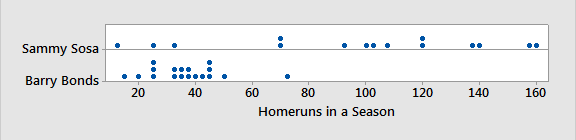
\includegraphics[width=0.5\linewidth]{images/q1.png}
 \end{figure}
\begin{enumerate}[label=\Alph*.]
    \item The mean homeruns is higher for Sosa than for Bonds.
    \item The standard deviation of homeruns is larger for Sosa than for Bonds.
    \item Both A and B
    \item Neither A nor B
    \item Cannot compare Sosa and Bonds.
\end{enumerate}

Use the dotplots to answer this question: We can compare baseball players Sammy Sosa and Barry Bonds by their batting averages. Which letter A-E is correct?
 \begin{figure}[h]
     \centering
     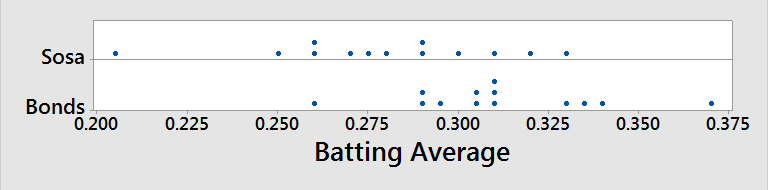
\includegraphics[width=0.5\linewidth]{images/q2.png}
 \end{figure}
\begin{enumerate}[label=\Alph*.]
    \item The typical batting average is higher for Sosa than for Bonds.
    \item Sosa is more likely than Bonds to have a batting average over 0.300.
    \item Both A and B
    \item Neither A nor B
    \item Cannot compare Sosa and Bonds.
\end{enumerate}

Use the story and the graph to answer this question: For Type A lightbulbs, the lifetime has $\mu = 3000 hours$ and$\sigma = 200 hours$. While for Type B lightbulbs, $\mu = 3000 hours$ and $\sigma = 250 hours$. 
\begin{figure}[h]
    \centering
    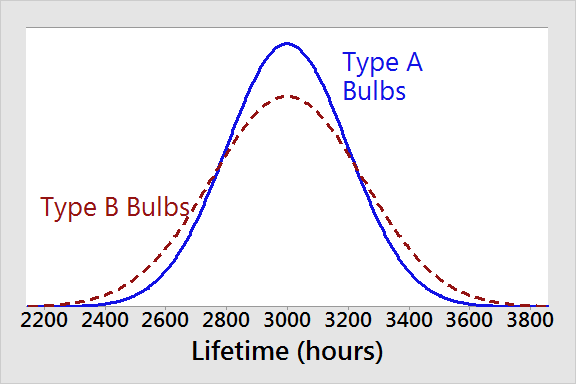
\includegraphics[width=0.5\linewidth]{images/q3.png}
\end{figure}
Which letter A-E is correct?
\begin{enumerate}[label=\Alph*.]
    \item Type A has a better chance of lasting over 3200 hours
    \item Type B has a better chance of lasting over 3200 hours
    \item Type A and Type B have the same average lifetime
    \item A and C
    \item B and C
\end{enumerate}

Use the dotplots to answer this question: The test scores for two Mars University courses are shown below. Which letter A-E is correct?
 \begin{figure}[h]
     \centering
     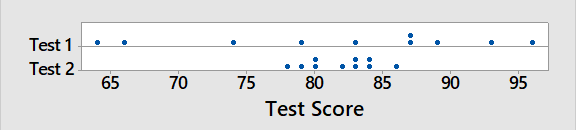
\includegraphics[width=0.5\linewidth]{images/q4.png}
 \end{figure}
\begin{enumerate}[label=\Alph*.]
    \item Test 1 has a smaller standard deviation; it’s more consistent and less variable
    \item Test 2 has a bigger standard deviation; it’s less consistent and more variable
    \item Test 2 has a wider spread than Test 1
    \item A, B, and C are all true
    \item A, B, and C are all false
\end{enumerate}

\textbf{Proportion/Percentage}

Use the graph to answer this question: What percentage of the 80 people answered “computer”? 
\begin{figure}[h]
    \centering
    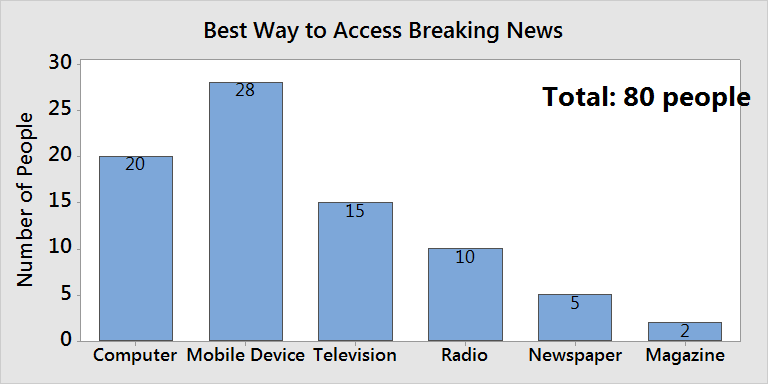
\includegraphics[width=0.5\linewidth]{images/q5.png}
\end{figure}
\begin{enumerate}[label=\Alph*.]
    \item 20\%
    \item 25\%
    \item 15\%
    \item 5\%
    \item 0\%
\end{enumerate}

Use the graph to answer this question: What percentage of the 80 people answered either “television” or “radio”?
\begin{figure}[h]
    \centering
    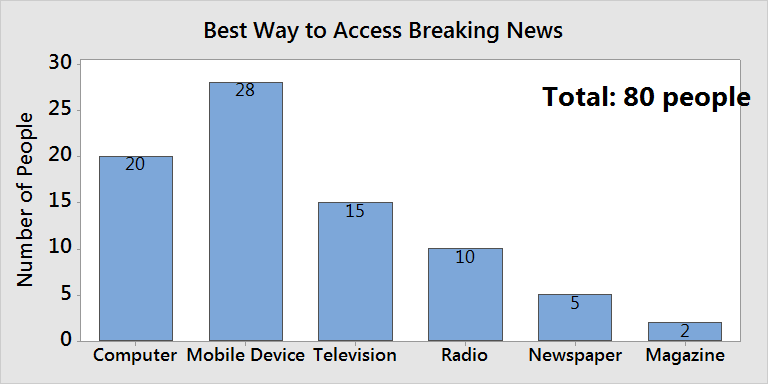
\includegraphics[width=0.5\linewidth]{images/q5.png}
\end{figure}
\begin{enumerate}[label=\Alph*.]
    \item 7\%
    \item 12\%
    \item 70\%
    \item 31\%
    \item 82\%
\end{enumerate}

Use the chart to answer this question: What percentage of the students travels to school by bus?
\begin{figure}[h]
    \centering
    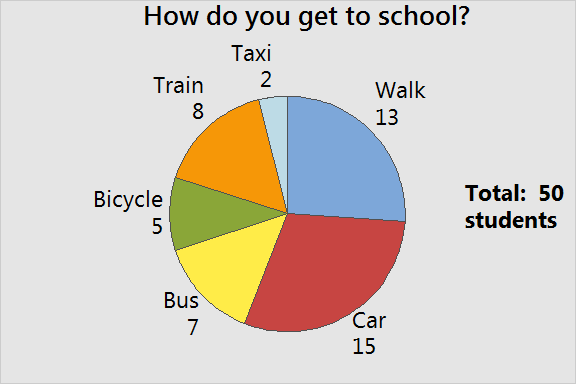
\includegraphics[width=0.5\linewidth]{images/q7.png}
\end{figure}
\begin{enumerate}[label=\Alph*.]
    \item 70\%
    \item 3\%
    \item 31\%
    \item 14\%
    \item None of the above
\end{enumerate}

Use the chart to answer this question: What proportion of students do NOT travel to school by car?
\begin{figure}[h]
    \centering
    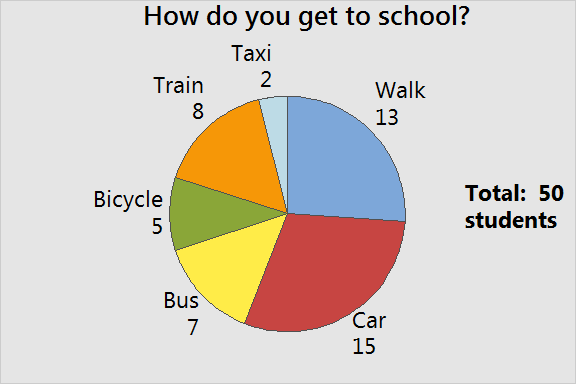
\includegraphics[width=0.5\linewidth]{images/q7.png}
\end{figure}
\begin{enumerate}[label=\Alph*.]
    \item 0.70
    \item 0.31
    \item 0.19
    \item 0.85
    \item None of the above
\end{enumerate}
 
\end{large}
\end{document}